\documentclass[12pt]{article}
\usepackage[utf8]{inputenc}
\usepackage{xcolor}
\usepackage[margin=1in]{geometry}
% \usepackage{graphicx}
\usepackage{float}
% \usepackage{textcomp}
% \usepackage{siunitx}
\usepackage{fancyhdr}
% \usepackage{amsmath, amssymb, amsthm}
\usepackage{tikz}
\usepackage{tikzpagenodes}
% \usepackage{eso-pic}
% \usepackage{enumerate}
\usepackage[colorlinks]{hyperref}
\hypersetup{
    colorlinks = true,
    linkcolor = blue,
    pdftitle={Graph Theory and Algorithms}
}
% \usepackage{lipsum}
% \usepackage{etoolbox}
\usepackage{bookmark}

% \makeatletter

% \renewcommand\float@endH{\@endfloatbox\vskip\intextsep
%   \if@flstyle\setbox\@currbox\float@makebox\columnwidth\fi
%   \box\@currbox\vskip\intextsep\relax\@doendpe}

% \patchcmd{\f@nch@head}{\rlap}{\color{white}\rlap}{}{}
% \patchcmd{\headrule}{\hrule}{\color{white}\hrule}{}{}
% \patchcmd{\f@nch@foot}{\rlap}{\color{white}\rlap}{}{}
% \patchcmd{\footrule}{\hrule}{\color{white}\hrule}{}{}

% \makeatother

%%% Header and footer
%%% ------------------------------------------
\pagestyle{fancy}
\fancyhf{}
\rhead{Summer of Science: Graph Theory}
% \fancyhead[L]{\nouppercase{\leftmark}}
\cfoot{\thepage}

%%% Macros
%%% ------------------------------------------
% \newcommand{\desctotoc}[4]{%
%   \addtocontents{toc}{\medskip\noindent\detokenize{#1}\leavevmode\par\medskip}
% }


\begin{document}


%%% Titlepage
%%% ------------------------------------------
\tikz[overlay] \node[opacity=1,inner sep=0pt] at (7.65,-12.5) {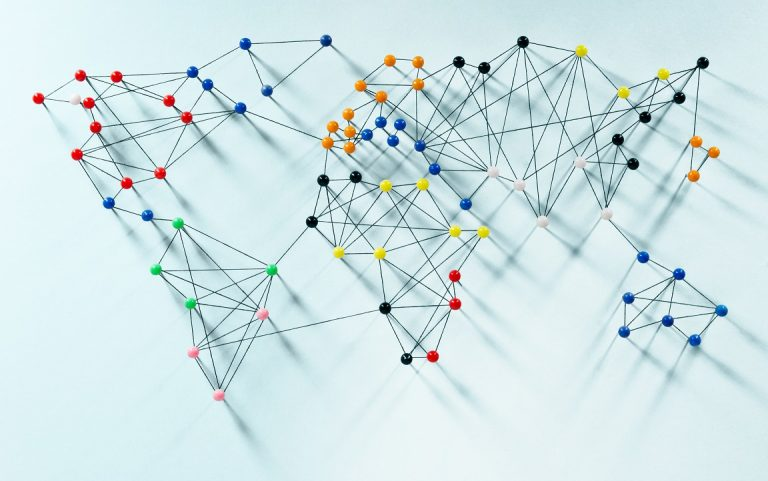
\includegraphics[width=\paperwidth]{./Graph-Theory-768x481.jpg}};
\vspace*{3cm}
\thispagestyle{empty}
	\begin{center}
	\textbf{\Huge{Graph Theory and Algorithms}}\\
	\textbf{\large{\\ An Introduction to the world of Graphs }}
	\end{center}
\vfill
	\begin{center}
	\large{\textbf{Devansh Jain,}\\
    Indian Institute of Technology, Bombay\\
    \vspace{0.5cm}
    (Mentor: Tathagat Verma)\\}
	\end{center}

\newpage

\pagenumbering{roman}
\begin{center}
\hspace{0pt}
    \tableofcontents
    \vfill
\hspace{0pt}
\end{center}

\newpage

\section*{Preface}
\addcontentsline{toc}{section}{Preface}
Preface
\subsubsection*{About the project}
adedsd
\subsubsection*{About the report}
sdsd
\subsubsection*{References and Acknowledgement}
sdfsd


\newpage
\pagenumbering{Roman}
\setcounter{page}{1}
{\color{black} \section*{MIT 6.042J}}
\addcontentsline{toc}{section}{MIT 6.042J}
\noindent
This course is available on OpenCourseWare MIT (ocw.mit.edu) as well as on Youtube channel MIT OpenCourseWare.\\
\subsubsection*{Course Instructor(s)}
Prof. Tom Leighton\\
Dr. Marten van Dijk
\subsubsection*{Course Description}
This course covers elementary discrete mathematics for computer science and engineering. It emphasizes mathematical definitions and proofs as well as applicable methods. Topics include formal logic notation, proof methods; induction, well-ordering; sets, relations; elementary graph theory; integer congruences; asymptotic notation and growth of functions; permutations and combinations, counting principles; discrete probability. Further selected topics may also be covered, such as recursive definition and structural induction; state machines and invariants; recurrences; generating functions.\\
\vspace{1cm}
In this report, I have included notes of Lectures 6 thru 11 which cover\\ 'Mathematical basics of Graph Theory'.\\
More detailed notes of the course are present \href{https://github.com/DEVANSH-DVJ/MIT-6.042J-18.062J-Fall-2010}{here}\\

\newpage
\pagenumbering{arabic}
\setcounter{page}{23}
\newpage
\begin{figure}[H]
    \centering
    \includegraphics[scale=0.25]{"./MIT 6.042J/MIT_6042J_023"}
\end{figure}
\newpage
\begin{figure}[H]
    \centering
    \includegraphics[scale=0.25]{"./MIT 6.042J/MIT_6042J_024"}
\end{figure}
\newpage
\begin{figure}[H]
    \centering
    \includegraphics[scale=0.25]{"./MIT 6.042J/MIT_6042J_025"}
\end{figure}
\newpage
\begin{figure}[H]
    \centering
    \includegraphics[scale=0.25]{"./MIT 6.042J/MIT_6042J_026"}
\end{figure}
\newpage
\begin{figure}[H]
    \centering
    \includegraphics[scale=0.25]{"./MIT 6.042J/MIT_6042J_027"}
\end{figure}
\newpage
\begin{figure}[H]
    \centering
    \includegraphics[scale=0.25]{"./MIT 6.042J/MIT_6042J_028"}
\end{figure}
\newpage
\begin{figure}[H]
    \centering
    \includegraphics[scale=0.25]{"./MIT 6.042J/MIT_6042J_029"}
\end{figure}
\newpage
\begin{figure}[H]
    \centering
    \includegraphics[scale=0.25]{"./MIT 6.042J/MIT_6042J_030"}
\end{figure}
\newpage
\begin{figure}[H]
    \centering
    \includegraphics[scale=0.25]{"./MIT 6.042J/MIT_6042J_031"}
\end{figure}
\newpage
\begin{figure}[H]
    \centering
    \includegraphics[scale=0.25]{"./MIT 6.042J/MIT_6042J_032"}
\end{figure}
\newpage
\begin{figure}[H]
    \centering
    \includegraphics[scale=0.25]{"./MIT 6.042J/MIT_6042J_033"}
\end{figure}
\newpage
\begin{figure}[H]
    \centering
    \includegraphics[scale=0.25]{"./MIT 6.042J/MIT_6042J_034"}
\end{figure}
\newpage
\begin{figure}[H]
    \centering
    \includegraphics[scale=0.25]{"./MIT 6.042J/MIT_6042J_035"}
\end{figure}
\newpage
\begin{figure}[H]
    \centering
    \includegraphics[scale=0.25]{"./MIT 6.042J/MIT_6042J_036"}
\end{figure}
\newpage
\begin{figure}[H]
    \centering
    \includegraphics[scale=0.25]{"./MIT 6.042J/MIT_6042J_037"}
\end{figure}
\newpage
\begin{figure}[H]
    \centering
    \includegraphics[scale=0.25]{"./MIT 6.042J/MIT_6042J_038"}
\end{figure}
\newpage
\begin{figure}[H]
    \centering
    \includegraphics[scale=0.25]{"./MIT 6.042J/MIT_6042J_039"}
\end{figure}
\newpage
\begin{figure}[H]
    \centering
    \includegraphics[scale=0.25]{"./MIT 6.042J/MIT_6042J_040"}
\end{figure}
\newpage
\begin{figure}[H]
    \centering
    \includegraphics[scale=0.25]{"./MIT 6.042J/MIT_6042J_041"}
\end{figure}
\newpage
\begin{figure}[H]
    \centering
    \includegraphics[scale=0.25]{"./MIT 6.042J/MIT_6042J_042"}
\end{figure}
\newpage
\begin{figure}[H]
    \centering
    \includegraphics[scale=0.25]{"./MIT 6.042J/MIT_6042J_043"}
\end{figure}
\newpage
\begin{figure}[H]
    \centering
    \includegraphics[scale=0.25]{"./MIT 6.042J/MIT_6042J_044"}
\end{figure}
\newpage
\begin{figure}[H]
    \centering
    \includegraphics[scale=0.25]{"./MIT 6.042J/MIT_6042J_045"}
\end{figure}
\newpage
\begin{figure}[H]
    \centering
    \includegraphics[scale=0.25]{"./MIT 6.042J/MIT_6042J_046"}
\end{figure}
\newpage
\begin{figure}[H]
    \centering
    \includegraphics[scale=0.25]{"./MIT 6.042J/MIT_6042J_047"}
\end{figure}
\newpage
\begin{figure}[H]
    \centering
    \includegraphics[scale=0.25]{"./MIT 6.042J/MIT_6042J_048"}
\end{figure}
\newpage
\begin{figure}[H]
    \centering
    \includegraphics[scale=0.25]{"./MIT 6.042J/MIT_6042J_049"}
\end{figure}
\newpage
\begin{figure}[H]
    \centering
    \includegraphics[scale=0.25]{"./MIT 6.042J/MIT_6042J_050"}
\end{figure}
\newpage
\begin{figure}[H]
    \centering
    \includegraphics[scale=0.25]{"./MIT 6.042J/MIT_6042J_051"}
\end{figure}
\newpage
\begin{figure}[H]
    \centering
    \includegraphics[scale=0.25]{"./MIT 6.042J/MIT_6042J_052"}
\end{figure}
\newpage
\begin{figure}[H]
    \centering
    \includegraphics[scale=0.25]{"./MIT 6.042J/MIT_6042J_053"}
\end{figure}
\newpage
\begin{figure}[H]
    \centering
    \includegraphics[scale=0.25]{"./MIT 6.042J/MIT_6042J_054"}
\end{figure}
\newpage
\begin{figure}[H]
    \centering
    \includegraphics[scale=0.25]{"./MIT 6.042J/MIT_6042J_055"}
\end{figure}
\newpage
\begin{figure}[H]
    \centering
    \includegraphics[scale=0.25]{"./MIT 6.042J/MIT_6042J_056"}
\end{figure}
\newpage
\begin{figure}[H]
    \centering
    \includegraphics[scale=0.25]{"./MIT 6.042J/MIT_6042J_057"}
\end{figure}
\newpage
\begin{figure}[H]
    \centering
    \includegraphics[scale=0.25]{"./MIT 6.042J/MIT_6042J_058"}
\end{figure}
\newpage
\begin{figure}[H]
    \centering
    \includegraphics[scale=0.25]{"./MIT 6.042J/MIT_6042J_059"}
\end{figure}
\newpage
\begin{figure}[H]
    \centering
    \includegraphics[scale=0.25]{"./MIT 6.042J/MIT_6042J_060"}
\end{figure}
\newpage
\begin{figure}[H]
    \centering
    \includegraphics[scale=0.25]{"./MIT 6.042J/MIT_6042J_061"}
\end{figure}
\newpage
\begin{figure}[H]
    \centering
    \includegraphics[scale=0.25]{"./MIT 6.042J/MIT_6042J_062"}
\end{figure}
\newpage
\begin{figure}[H]
    \centering
    \includegraphics[scale=0.25]{"./MIT 6.042J/MIT_6042J_063"}
\end{figure}
\newpage
\begin{figure}[H]
    \centering
    \includegraphics[scale=0.25]{"./MIT 6.042J/MIT_6042J_064"}
\end{figure}
\newpage
\begin{figure}[H]
    \centering
    \includegraphics[scale=0.25]{"./MIT 6.042J/MIT_6042J_065"}
\end{figure}
\newpage
\begin{figure}[H]
    \centering
    \includegraphics[scale=0.25]{"./MIT 6.042J/MIT_6042J_066"}
\end{figure}
\newpage
\begin{figure}[H]
    \centering
    \includegraphics[scale=0.25]{"./MIT 6.042J/MIT_6042J_067"}
\end{figure}
\newpage
\begin{figure}[H]
    \centering
    \includegraphics[scale=0.25]{"./MIT 6.042J/MIT_6042J_068"}
\end{figure}
\newpage
\begin{figure}[H]
    \centering
    \includegraphics[scale=0.25]{"./MIT 6.042J/MIT_6042J_069"}
\end{figure}
\newpage
\begin{figure}[H]
    \centering
    \includegraphics[scale=0.25]{"./MIT 6.042J/MIT_6042J_070"}
\end{figure}
\newpage
\begin{figure}[H]
    \centering
    \includegraphics[scale=0.25]{"./MIT 6.042J/MIT_6042J_071"}
\end{figure}
\newpage
\begin{figure}[H]
    \centering
    \includegraphics[scale=0.25]{"./MIT 6.042J/MIT_6042J_072"}
\end{figure}
\newpage
\begin{figure}[H]
    \centering
    \includegraphics[scale=0.25]{"./MIT 6.042J/MIT_6042J_073"}
\end{figure}
\newpage
\begin{figure}[H]
    \centering
    \includegraphics[scale=0.25]{"./MIT 6.042J/MIT_6042J_074"}
\end{figure}
\newpage
\begin{figure}[H]
    \centering
    \includegraphics[scale=0.25]{"./MIT 6.042J/MIT_6042J_075"}
\end{figure}
\newpage
\begin{figure}[H]
    \centering
    \includegraphics[scale=0.25]{"./MIT 6.042J/MIT_6042J_076"}
\end{figure}
\newpage
\begin{figure}[H]
    \centering
    \includegraphics[scale=0.25]{"./MIT 6.042J/MIT_6042J_077"}
\end{figure}


\newpage
\pagenumbering{Roman}
\setcounter{page}{2}
{\color{black} \section*{MIT 6.006}}
\addcontentsline{toc}{section}{MIT 6.006}
\noindent
This course is available on OpenCourseWare MIT (ocw.mit.edu) as well as on Youtube channel MIT OpenCourseWare.\\
\subsubsection*{Course Instructor(s)}
Prof. Erik Demaine\\
Prof. Srini Devadas
\subsubsection*{Course Description}
This course provides an introduction to mathematical modeling of computational problems. It covers the common algorithms, algorithmic paradigms, and data structures used to solve these problems. The course emphasizes the relationship between algorithms and programming, and introduces basic performance measures and analysis techniques for these problems.\\
\vspace{1cm}
In this report, I have included my notes of Lectures 13 thru 18 which cover\\ 'Basic algorithms of Graph Theory'.\\
More detailed notes of the course are present \href{https://github.com/devansh-dvj/MIT-6.006-Fall-2011}{here}\\

\newpage
\pagenumbering{arabic}
\setcounter{page}{95}
\newpage
\begin{figure}[H]
    \centering
    \includegraphics[scale=0.25]{"./MIT-6.006/MIT-6006-095"}
\end{figure}
\newpage
\begin{figure}[H]
    \centering
    \includegraphics[scale=0.25]{"./MIT-6.006/MIT-6006-096"}
\end{figure}
\newpage
\begin{figure}[H]
    \centering
    \includegraphics[scale=0.25]{"./MIT-6.006/MIT-6006-097"}
\end{figure}
\newpage
\begin{figure}[H]
    \centering
    \includegraphics[scale=0.25]{"./MIT-6.006/MIT-6006-098"}
\end{figure}
\newpage
\begin{figure}[H]
    \centering
    \includegraphics[scale=0.25]{"./MIT-6.006/MIT-6006-099"}
\end{figure}
\newpage
\begin{figure}[H]
    \centering
    \includegraphics[scale=0.25]{"./MIT-6.006/MIT-6006-100"}
\end{figure}
\newpage
\begin{figure}[H]
    \centering
    \includegraphics[scale=0.25]{"./MIT-6.006/MIT-6006-101"}
\end{figure}
\newpage
\begin{figure}[H]
    \centering
    \includegraphics[scale=0.25]{"./MIT-6.006/MIT-6006-102"}
\end{figure}
\newpage
\begin{figure}[H]
    \centering
    \includegraphics[scale=0.25]{"./MIT-6.006/MIT-6006-103"}
\end{figure}
\newpage
\begin{figure}[H]
    \centering
    \includegraphics[scale=0.25]{"./MIT-6.006/MIT-6006-104"}
\end{figure}
\newpage
\begin{figure}[H]
    \centering
    \includegraphics[scale=0.25]{"./MIT-6.006/MIT-6006-105"}
\end{figure}
\newpage
\begin{figure}[H]
    \centering
    \includegraphics[scale=0.25]{"./MIT-6.006/MIT-6006-106"}
\end{figure}
\newpage
\begin{figure}[H]
    \centering
    \includegraphics[scale=0.25]{"./MIT-6.006/MIT-6006-107"}
\end{figure}
\newpage
\begin{figure}[H]
    \centering
    \includegraphics[scale=0.25]{"./MIT-6.006/MIT-6006-108"}
\end{figure}
\newpage
\begin{figure}[H]
    \centering
    \includegraphics[scale=0.25]{"./MIT-6.006/MIT-6006-109"}
\end{figure}
\newpage
\begin{figure}[H]
    \centering
    \includegraphics[scale=0.25]{"./MIT-6.006/MIT-6006-110"}
\end{figure}
\newpage
\begin{figure}[H]
    \centering
    \includegraphics[scale=0.25]{"./MIT-6.006/MIT-6006-111"}
\end{figure}
\newpage
\begin{figure}[H]
    \centering
    \includegraphics[scale=0.25]{"./MIT-6.006/MIT-6006-112"}
\end{figure}
\newpage
\begin{figure}[H]
    \centering
    \includegraphics[scale=0.25]{"./MIT-6.006/MIT-6006-113"}
\end{figure}
\newpage
\begin{figure}[H]
    \centering
    \includegraphics[scale=0.25]{"./MIT-6.006/MIT-6006-114"}
\end{figure}
\newpage
\begin{figure}[H]
    \centering
    \includegraphics[scale=0.25]{"./MIT-6.006/MIT-6006-115"}
\end{figure}
\newpage
\begin{figure}[H]
    \centering
    \includegraphics[scale=0.25]{"./MIT-6.006/MIT-6006-116"}
\end{figure}
\newpage
\begin{figure}[H]
    \centering
    \includegraphics[scale=0.25]{"./MIT-6.006/MIT-6006-117"}
\end{figure}
\newpage
\begin{figure}[H]
    \centering
    \includegraphics[scale=0.25]{"./MIT-6.006/MIT-6006-118"}
\end{figure}
\newpage
\begin{figure}[H]
    \centering
    \includegraphics[scale=0.25]{"./MIT-6.006/MIT-6006-119"}
\end{figure}
\newpage
\begin{figure}[H]
    \centering
    \includegraphics[scale=0.25]{"./MIT-6.006/MIT-6006-120"}
\end{figure}
\newpage
\begin{figure}[H]
    \centering
    \includegraphics[scale=0.25]{"./MIT-6.006/MIT-6006-121"}
\end{figure}
\newpage
\begin{figure}[H]
    \centering
    \includegraphics[scale=0.25]{"./MIT-6.006/MIT-6006-122"}
\end{figure}
\newpage
\begin{figure}[H]
    \centering
    \includegraphics[scale=0.25]{"./MIT-6.006/MIT-6006-123"}
\end{figure}
\newpage
\begin{figure}[H]
    \centering
    \includegraphics[scale=0.25]{"./MIT-6.006/MIT-6006-124"}
\end{figure}
\newpage
\begin{figure}[H]
    \centering
    \includegraphics[scale=0.25]{"./MIT-6.006/MIT-6006-125"}
\end{figure}
\newpage
\begin{figure}[H]
    \centering
    \includegraphics[scale=0.25]{"./MIT-6.006/MIT-6006-126"}
\end{figure}
\newpage
\begin{figure}[H]
    \centering
    \includegraphics[scale=0.25]{"./MIT-6.006/MIT-6006-127"}
\end{figure}
\newpage
\begin{figure}[H]
    \centering
    \includegraphics[scale=0.25]{"./MIT-6.006/MIT-6006-128"}
\end{figure}
\newpage
\begin{figure}[H]
    \centering
    \includegraphics[scale=0.25]{"./MIT-6.006/MIT-6006-129"}
\end{figure}
\newpage
\begin{figure}[H]
    \centering
    \includegraphics[scale=0.25]{"./MIT-6.006/MIT-6006-130"}
\end{figure}
\newpage
\begin{figure}[H]
    \centering
    \includegraphics[scale=0.25]{"./MIT-6.006/MIT-6006-131"}
\end{figure}
\newpage
\begin{figure}[H]
    \centering
    \includegraphics[scale=0.25]{"./MIT-6.006/MIT-6006-132"}
\end{figure}
\newpage
\begin{figure}[H]
    \centering
    \includegraphics[scale=0.25]{"./MIT-6.006/MIT-6006-133"}
\end{figure}


\newpage
\pagenumbering{Roman}
\setcounter{page}{3}
{\color{black} \section*{Further}}
\addcontentsline{toc}{section}{Further}
About it


\end{document}
